\begin{figure}
    \begin{center}
    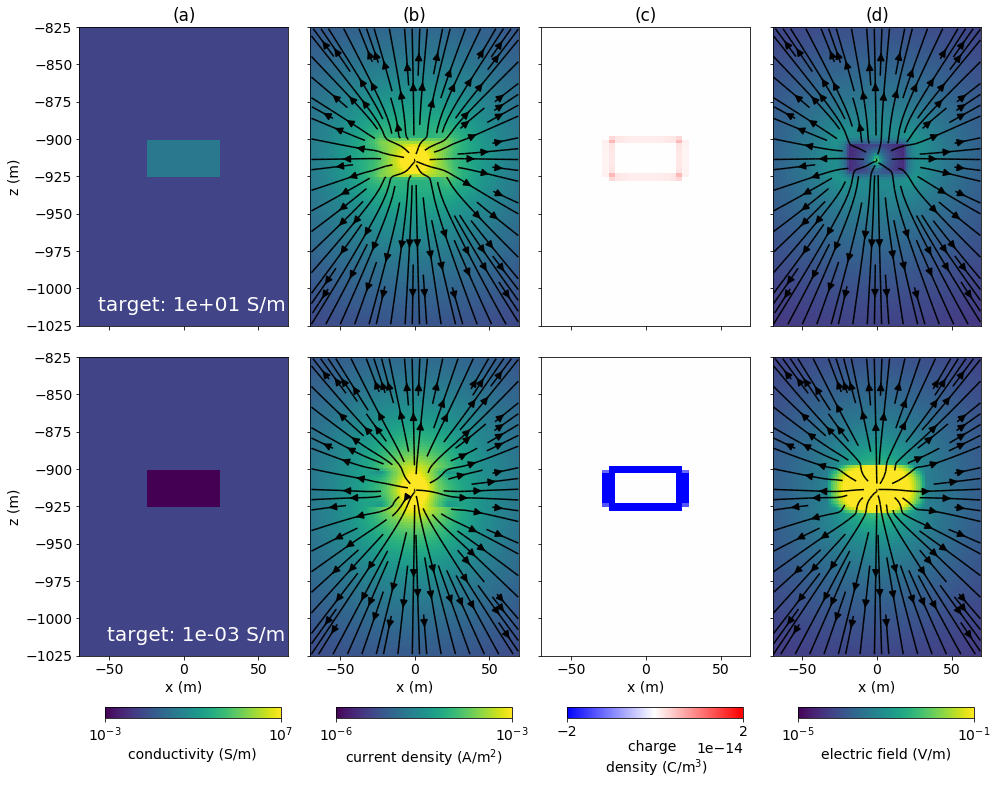
\includegraphics[width=\textwidth]{figures/uncased_target_physics.png}
    \end{center}
\caption{
    Cross section showing: (a) electrical conductivity, (b) current density, (c) charge density, and
    (d) electric field for a DC resistivity experiment with a conductive target (top) and a resistive target
    (bottom). The positive electrode is positioned at 912.5m depth.
    No casing is included in this simulation. Note that the colorbars for the charge density (c) and electric field (d)
    are different than those used in Figure \ref{fig:target_physics}. For the resistive target, the colorbar is saturated,
    the charge density over the resistive target is on the order of $10^{-13}$ C/m$^3$.
}
\label{fig:uncased_target_physics}
\end{figure}
